\section{Основная часть}

Основная часть данной работы состоит из подготовки данных, обучения модели детектирования объектов, применения алгоритма трекинга, проведения постобработки и анализа полученных результатов.

\subsection{Подготовка данных}

В задаче классификации нередко возникают ситуации, когда в обучающей выборке доли объектов различных классов существенно разнятся, создавая так называемую проблему несбалансированности классов \cite{9-1}, негативно влияющую на результат работы моделей.

У используемого в данной работе датасета VisDrone существует две особенности, вызывающие проблемы с детектированием: несбалансированность классов и малое количество аннотаций для сценариев плотного расположения групп объектов малого размера.

Для решения первой проблемы были использованы аугментации для искусственного увеличения количества изображений с объектами малопредставленных классов, идея чего вдохновлена методом перебалансировки данных Synthetic Minority Over-Sampling Technique (SMOTE) \cite{9-2}, предполагающем увеличение объема миноритарных классов в дополнение к уменьшению объема мажоритарных классов. Так как при классическом использовании удаления объектов преобладающих классов возможно удаление ключевых сценариев \cite{9-3}, в работе использовано только искусственное увеличение количества объектов малопредставленных классов.

Был проведен анализ датасета с целью выявления для каждого класса видеопоследовательностей с наибольшим количеством объектов из него. Для каждой такой видеопоследовательности были найдены кадры с наиболее плотным скоплением объектов из соответствующего класса, как показано на Рис. \ref{img:9-1}. Далее по координатам из аннотаций найденные области были вырезаны и увеличены, после чего к ним были применены операции аугментации во избежание переобучения модели на одинаковых кадрах, а именно различные повороты, позволившие значительно увеличить количество объектов в малопредставленных классах, как на Рис. \ref{img:9-2} и \ref{img:9-3}.

\vspace{0.5cm}

\begin{figure}[ht]
    \centering
    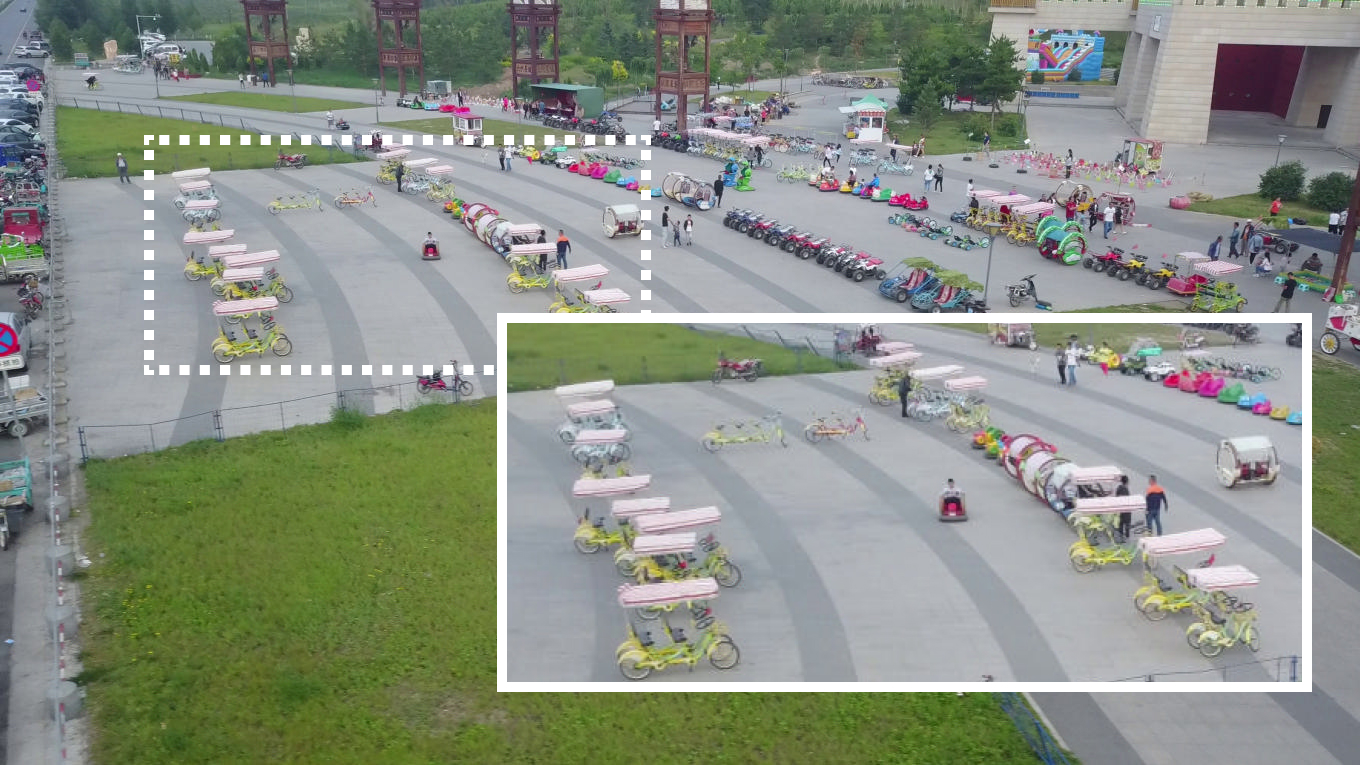
\includegraphics[width=0.85\textwidth]{9-1}
    \caption{Пример области с объектами малопредставленного класса}
    \label{img:9-1}
\end{figure}

\begin{figure}[ht]
    \centering
    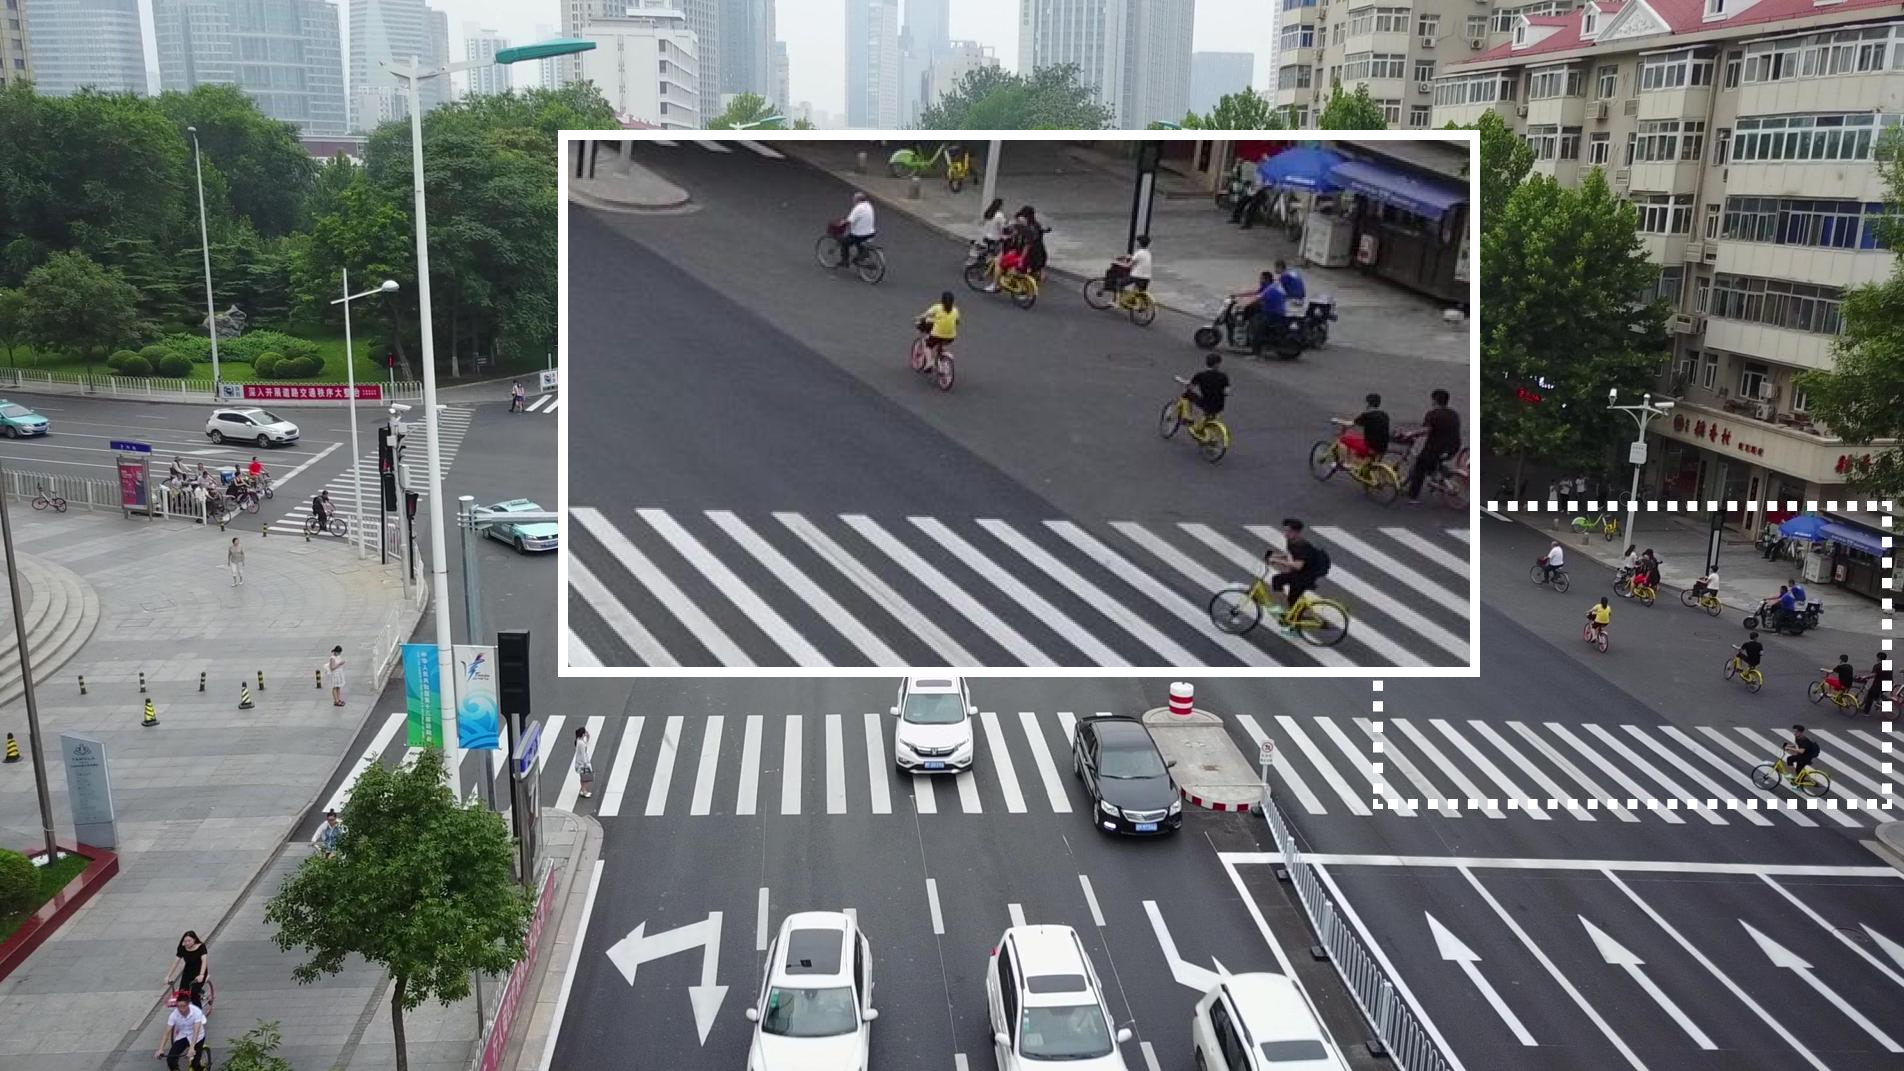
\includegraphics[width=0.85\textwidth]{9-2}
    \caption{Найденная область с объектами малопредставленного класса}
    \label{img:9-2}
\end{figure}

\begin{figure}[ht]
    \centering
    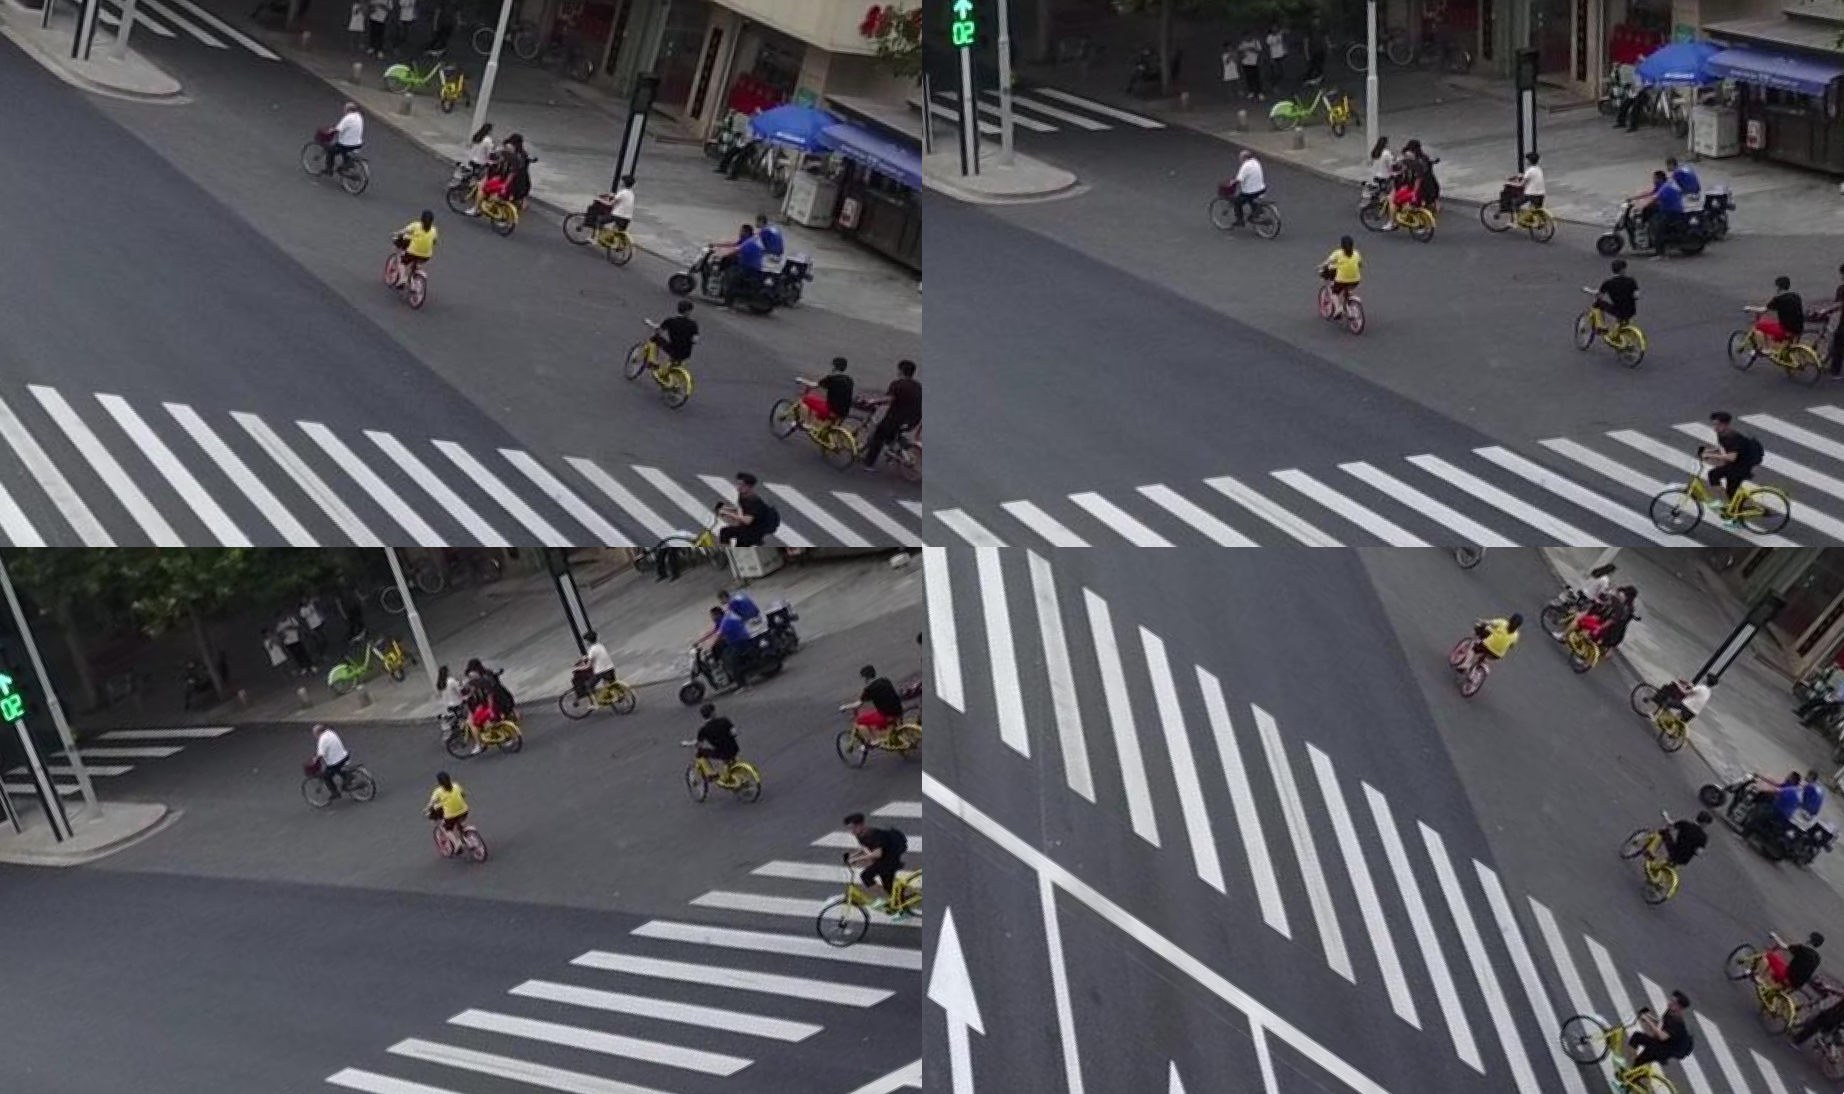
\includegraphics[width=0.85\textwidth]{9-3}
    \caption{Аугментации поворотами полученной области}
    \label{img:9-3}
\end{figure}

Проделанная работа помогла уравновесить количество объектов в классах, несбалансированность которых была представлена на Рис. \ref{img:3-3}, результат чего можно увидеть на Рис. \ref{img:9-4}.

\begin{figure}[ht]
    \centering
    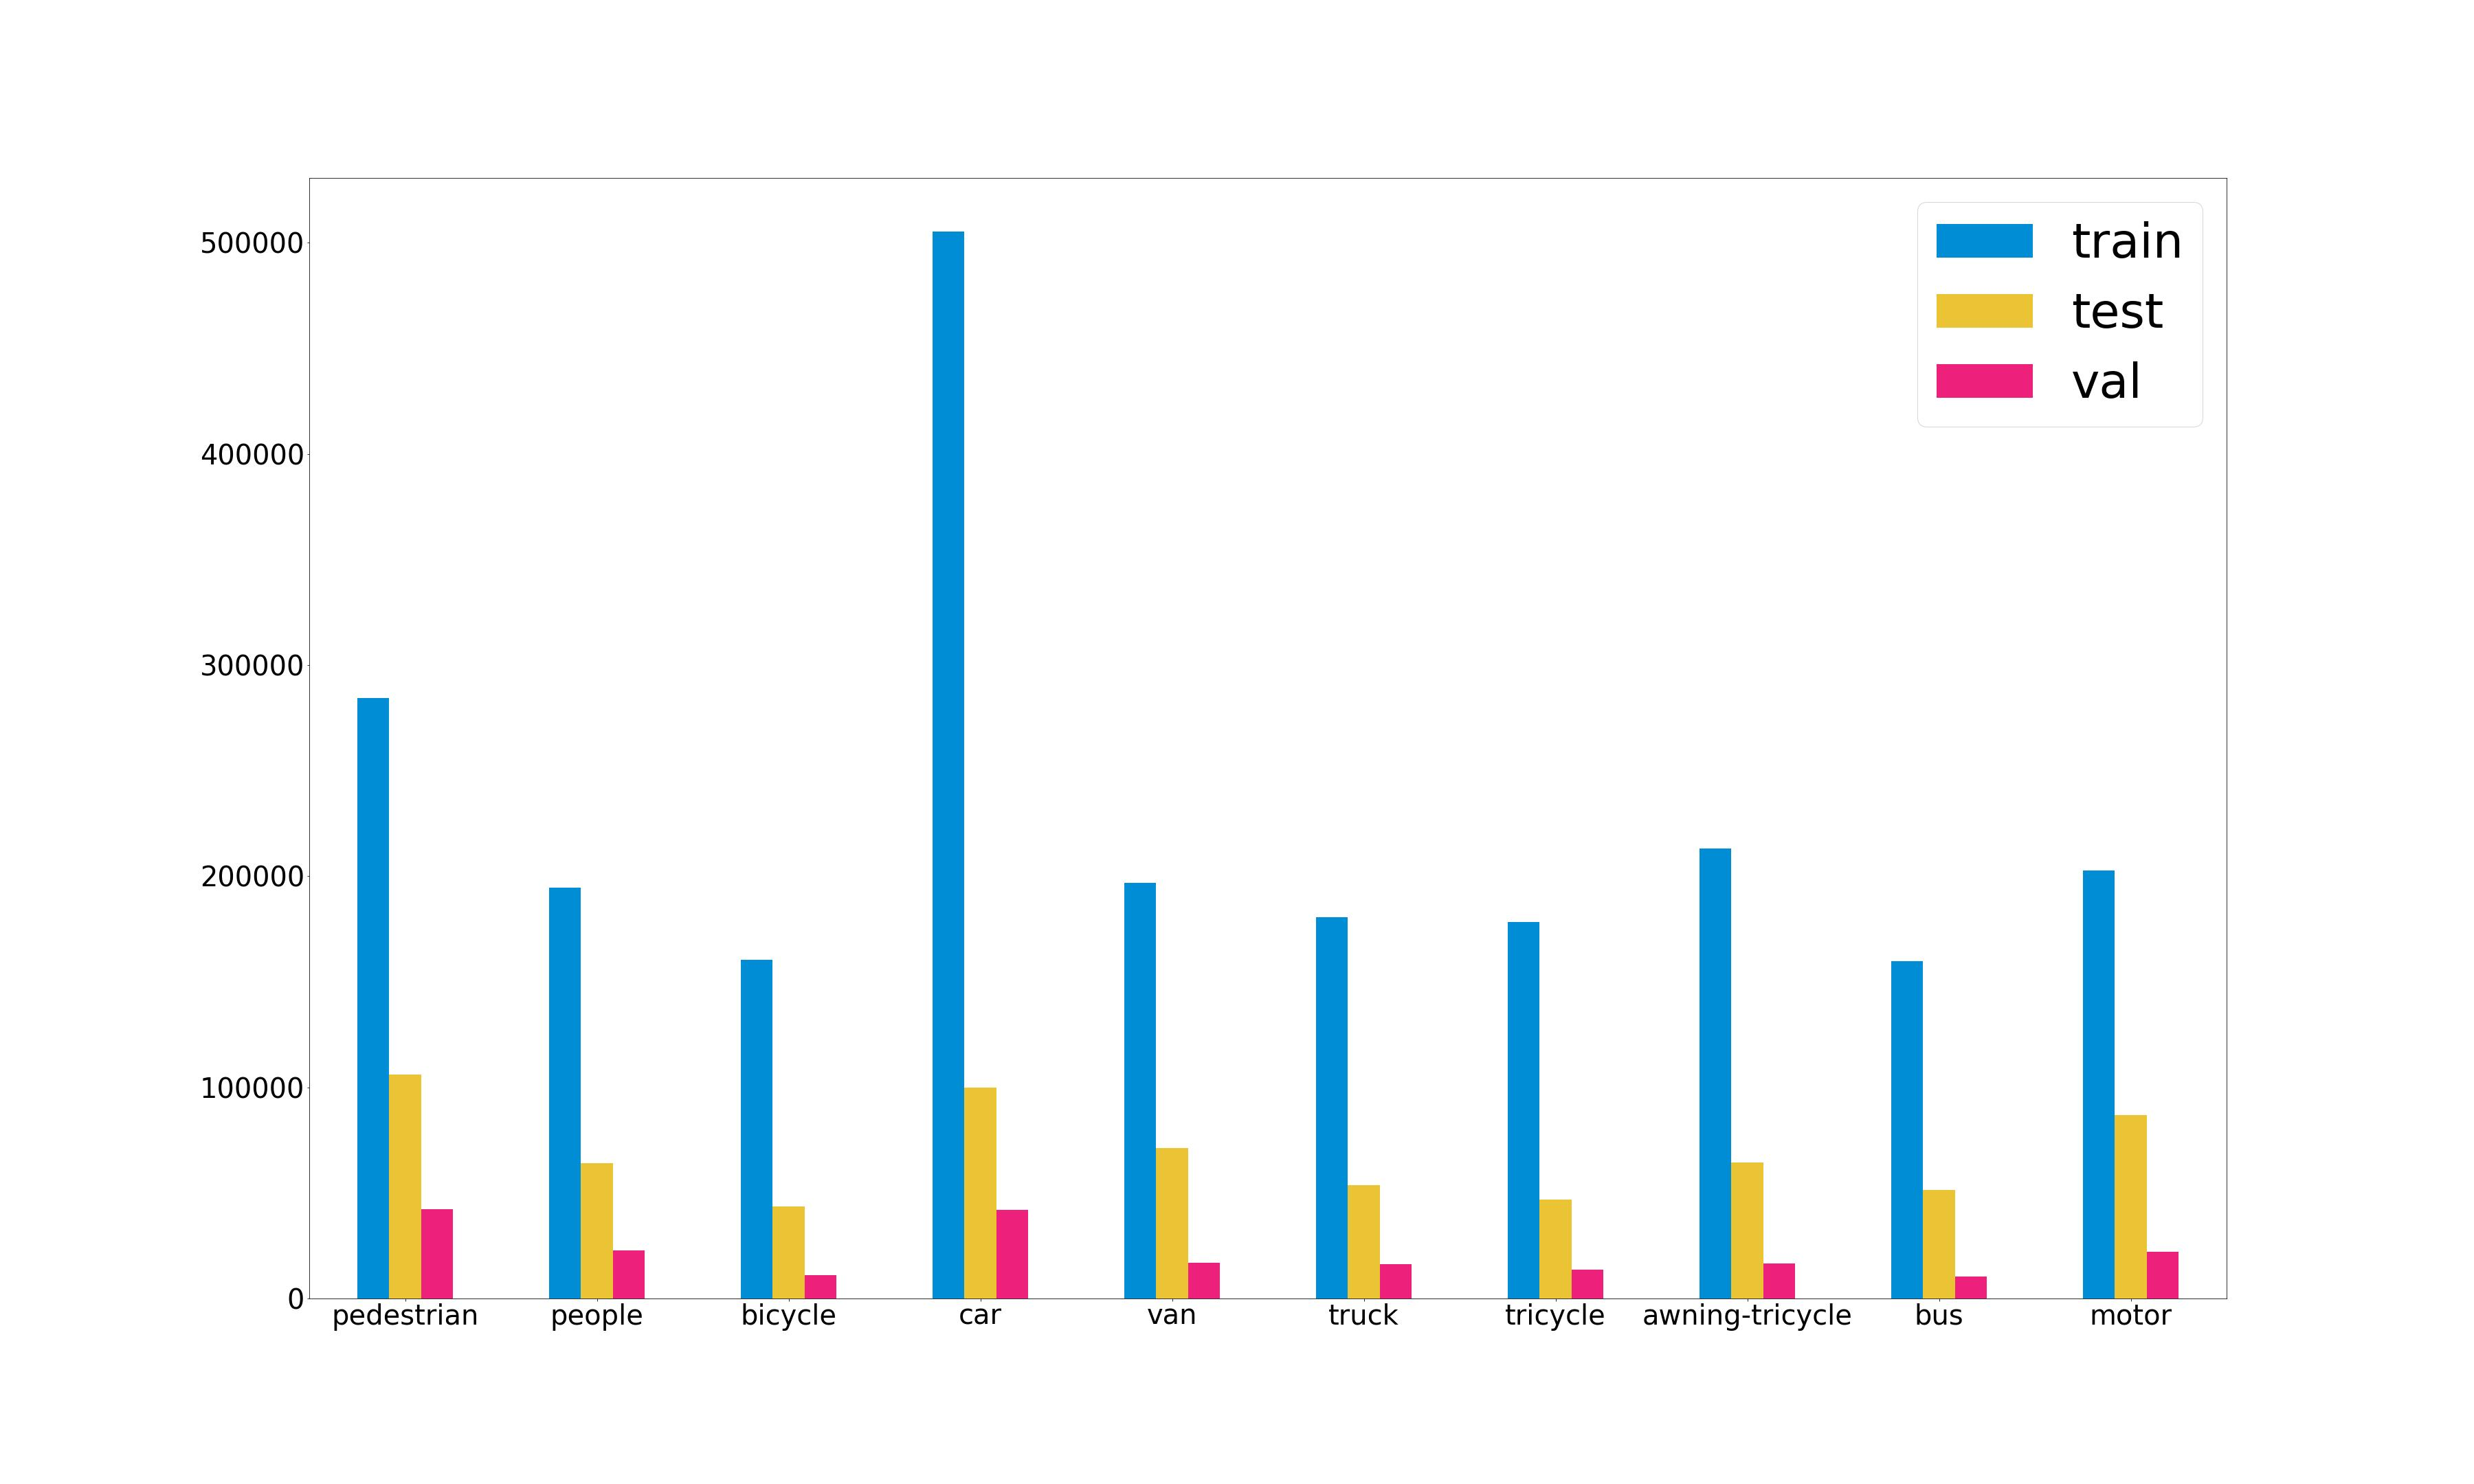
\includegraphics[width=0.85\textwidth]{9-4}
    \caption{Новое распределение объектов по классам}
    \label{img:9-4}
\end{figure}

Для решения второй вышеприведенной проблемы был дополнительно использован датасет UAVDT по причине наличия в нем множества сценариев плотного расположения объектов. После проведения анализа датасета были выбраны видеопоследовательности с наибольшим количеством объектов в кадре, как на Рис. \ref{img:9-5}, большая часть которых отобрана по наличию в атрибутах датасета меток о высокой точке обзора. 

\vspace{0.5cm}

\begin{figure}[ht]
    \centering
    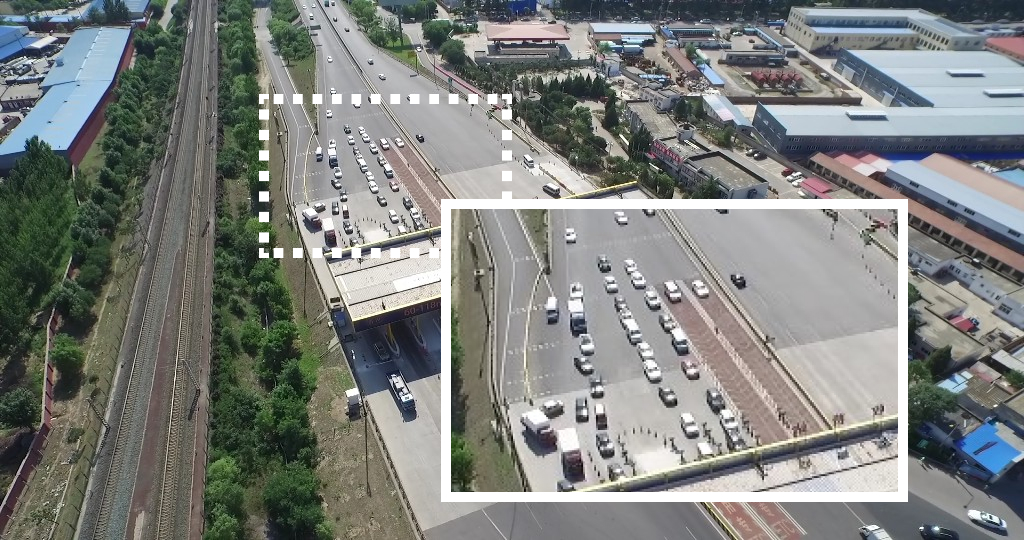
\includegraphics[width=0.85\textwidth]{9-5}
    \caption{Пример области с плотным расположением объектов малого размера}
    \label{img:9-5}
\end{figure}
